\section {Réactualisation du système}

\subsection*{Cockburn de la réactualisation du système}
\noindent 


\begin{tabular}{|p{1.1in}|p{1.1in}|p{1.5in}|p{1.5in}|} \hline 
\textbf{Cas d'utilisation }& \multicolumn{3}{|p{1in}|}{\textbf{Réactualiser}} \\ \hline 
\textbf{}\textbf{Acteur} & \multicolumn{3}{|p{3.2in}|}{Objectif Utilisateur} \\ \hline 
\textbf{Parties prenantes et intérêts} & \multicolumn{3}{|p{4in}|}{~Réactualisation régulière et systématique du système :\newline  mise à jour des fiches contexte, et ajout des nouveaux éléments au fur et à mesure (au moins une fois par jour),\newline  examen du calendrier à venir, des sujets en cours et en réserve, de l'échéancier, mise à jour des listes et dossiers, prospective, nettoyage de l'inutile(au minimum hebdomadaire)} \\ \hline 
\textbf{Niveau} & \multicolumn{3}{|p{3.2in}|}{~Utilisateur} \\ \hline 
\textbf{Portée} & \multicolumn{3}{|p{3.2in}|}{~Système GTD} \\ \hline 
\textbf{Pré-conditions} & \multicolumn{3}{|p{3.2in}|}{~} \\ \hline 
\textbf{Post-conditions} & \multicolumn{3}{|p{4in}|}{~Les informations sont mises à jour dans le système.} \\ \hline 
\textbf{Scénario nominal} & \textbf{Etapes} &  \multicolumn{2}{|p{2.5in}|}{\textbf{Action}} \\ \hline 
\textbf{~} & 1  &  \multicolumn{2}{|p{3in}|}{Mise à jour des contextes} \\ \hline 
\textbf{} & 2 & \multicolumn{2}{|p{3in}|}{Ajout des nouvelles informations (postit, système d'information)}  \\ \hline 
\textbf{} & 2 & \multicolumn{2}{|p{3in}|}{Examen de l'échéancier et de l'agenda}  \\ \hline 
\textbf{} & 2 & \multicolumn{2}{|p{3in}|}{Suppression des tâches effectuées, des ressources plus utilisées...}  \\ \hline 
\textbf{Extensions} & \textbf{Etapes} & \textbf{Condition} & \textbf{Action} \\ \hline 
\textbf{}\textbf{~} & * & A tout moment & ~L'utilisateur peut quitter l'action en cours \\ \hline 
\textbf{Contraintes} & \textbf{Type} & \textbf{Description} & ~ \\ \hline 
\textbf{~} & ~Correction &\multicolumn{2}{|p{3in}|}{Les informations ennoncées sont réelles et correctes} \\ \hline 
\textbf{Priorité} & \multicolumn{3}{|p{3.2in}|}{~Très Elevée (5/5)} \\ \hline 
\textbf{Performance} & \multicolumn{3}{|p{3.2in}|}{~} \\ \hline 
\textbf{Fréquences} & \multicolumn{3}{|p{3.2in}|}{~Au moins une fois par jour} \\ \hline 
\end{tabular}







\subsection*{Scenario de la réactualisation du système}

\begin{figure}[H]
	\begin{center}
	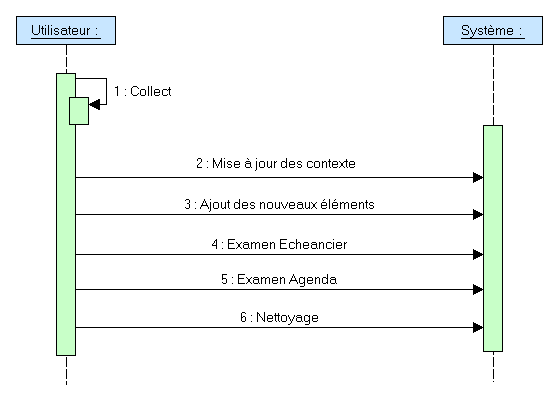
\includegraphics[scale=0.5]{diagrams/ScenarRevue.png}
	\caption{Diagramme UML  - Scénario \textit{Revue}}
	\end{center}
	\end{figure}
	
	\bigskip
	
	Le scénario du cas d'utilisation \textit{Revue} utilise celui de Collect. En effet, la revue est un examen, un point sur là où nous sommes au moment présent. On effectue donc de nouveau un collect pour ajouter de nouveaux élements s'il y a lieu puis on passe aux étapes de revue à proprement parler : \\
	\begin{itemize}
\item L'utilisateur mets a jour le contexte des tâches existantes s'il a changé,
\item il ajoute les nouveaux élements,
\item il examine l'écheancier,
\item il examine l'agenda,
\item enfin, il "nettoie" le système des tâches déja effectuées, des ressources qui ne seront plus utilisées..
\end{itemize}
	
\subsection*{Diagramme d'objets}

\subsubsection {Avant \textit{la réactualisation du système}}

\begin{figure}[H]
	\begin{center}
	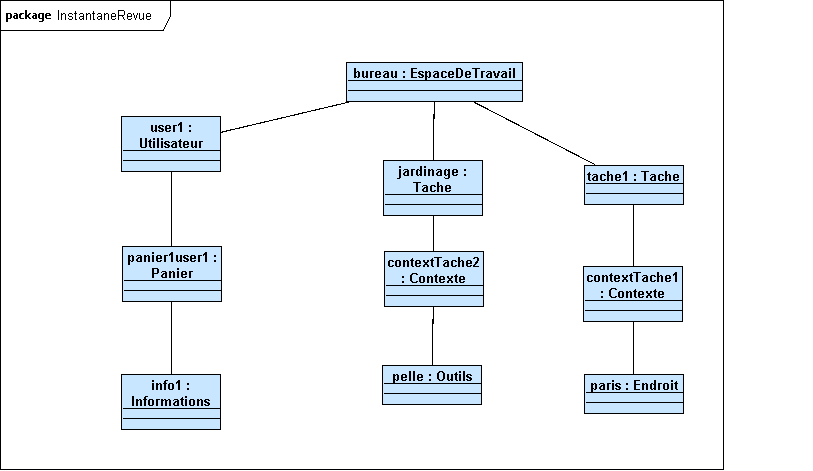
\includegraphics[scale=0.5]{diagrams/InstantaneRevueBefore.png}
	\caption{Diagramme d'objets UML  - Avant \textit{Revue} }
	\end{center}
	\end{figure}
	
	\bigskip

	On a ici le snapshot d'un système en cours d'execution. En effet, l'utilisateur possède un EspaceDeTravail (bureau) qui possède deux tâches préalablement enregistrées (lors du \textit{Process} ) :\\
	\begin{itemize}
\item jardinage dont le contexte possède la propriété qui spécifie l'outil : une pelle.
\item tache1 dont le contexte possède la propriété qui spécifie l'endroit : paris.
\end{itemize}


\subsubsection {Après \textit{la réactualisation du système}}

\begin{figure}[H]
	\begin{center}
	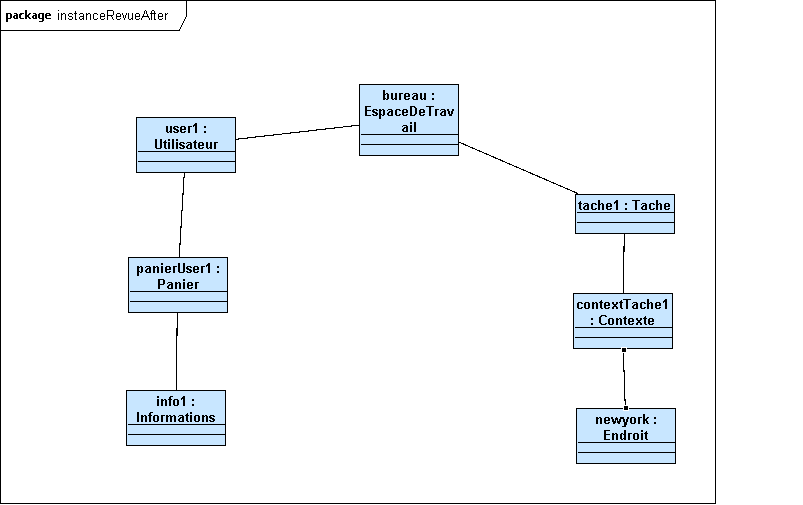
\includegraphics[scale=0.5]{diagrams/InstantaneRevueAfter.png}
	\caption{Diagramme d'objets UML  - Après \textit{Revue}}
	\end{center}
\end{figure}
	
	\bigskip

	Apres \textit{Revue}, on admet que le lieu du shopping a changé suite à l'annulation d'un ami. Ainsi, après la revue le lieu a été mis à jour, il passe de paris à newyork. De plus, la tâche jardinage ayant été réalisée entre cette revue et la précédente, nous l'avons supprimée.
